% Netzwerkanltung für die Studentenstadt Freimann
% Tex initially created by Maximilian Engelhardt <maximilian.engelhardt@stusta.mhn.de>

%\documentclass[a4paper,12pt,draft]{scrartcl}
\documentclass[a4paper,12pt]{scrartcl}

\usepackage[utf8]{inputenc}
\usepackage{ngerman}
\usepackage{eurosym}
\usepackage{tabularx}
\usepackage[pdftex,final]{graphicx}
\usepackage{wrapfig}
\usepackage[top=1.5cm,bottom=2.5cm,left=1.5cm,right=1.5cm]{geometry}
%\usepackage[margin=2cm]{geometry}
\usepackage{hyperref}


\title{Wohnanlage Studentenstadt Freimann:\\
       Anleitung zum Einrichten des Internetzugangs}
%\date{\today}

\begin{document}

\maketitle

\begin{figure}[t!]
   \centering
   \vspace{-20pt}
   
\includegraphics[width=0.8\textwidth,keepaspectratio]{Bilder/StuStaNet_Logo}
   \vspace{-40pt}
\end{figure}

\section*{Allgemeine Informationen zum Netzwerkanschluss}

Dies ist eine Beschreibung, wie Sie ihren Computer an das Netzwerk der Studentenstadt anschließen. Lesen Sie vorher die Benutzerordnung gründlich durch, die Sie mit ihrem Mietvertrag erhalten haben.
\\
\\
Sie benötigen einen Computer mit LAN-Kabelanschluss, und ein LAN-Kabel zum Anschluss des Computers an der im Zimmer angebrachten Netzwerkdose. Diese Kabel können im Fachhandel oder auch beim StuStaNet e.V. während der Sprechstunde (siehe weiter unten) erworben werden.
\\
\\
Jeder, der seinen Computer an das Netzwerk der Studentenstadt anschließt, ist dafür verantwortlich, dass dadurch keine anderen Rechner im Netzwerk gefährdet werden. Dazu gehört seinen Rechner vor Viren oder anderer Schadsoftware zu schützen.
Der Stustanet~e.V. betreibt eine Schadsoftwareerkennung, die Anschlüsse bei Auffälligkeiten aufgrund von Virenbefall vorübergehend sperrt.
\\
\begin{bfseries}
	\\Bei wiederholter Virendiagnose wird der entsprechende Anschluss dauerhaft gesperrt.
\end{bfseries}
\\
\\
In der StuSta gibt es kein zentrales WLAN, allerdings kann jeder selbst einen Access Point betreiben. In den Einstellungen des Routers/AP muss eine der Zimmer-IPs, sowie Gateway, Subnetzmakse und DNS eingestellt werden. Der StuStaNet e.V. verkauft für die StuSta passend vorkonfigurierte Geräte in der Sprechstunde (nur an Mitglieder).



%\pagebreak

\section*{Mitgliedschaft StuStaNet e.V.}
Es gibt zwei Möglichkeiten im Internet zu surfen. Die Standard-Variante ist der Zugang über den Proxyserver. Allerdings muss dieser bei jeder Applikation eingestellt werden, falls dies unterstützt wird. Einige Software unterstützt zudem die ohne Mitgliedschaft nötige manuelle Proxyeinrichtung nicht, das heißt, dass zum Beispiel für Programme wie WhatsApp oder League of Legends eine Mitgliedschaft notwendig ist, damit diese funktionieren.\\
\\
Die andere Möglichkeit ist über unser NAT-Gateway. Dieses und einige andere Dienste\footnote{http://wiki.stusta.de/Dienste} stehen für Mitglieder des StuStaNet e.V. zur Verfügung. Die Konfiguration des Proxys kann dann entfallen.
Für die Mitgliedschaft fällt eine \textbf{einmalige} Aufnahmegebühr von \EUR{20} an. Um Mitglied zu werden, registrieren Sie sich bitte vorab unter \mbox{\url{https://reg.stustanet.de}} und kommen Sie zu einer unserer Sprechstunden in Haus 10, Zimmer 1002 (Kellergeschoss). Die Adresse des Hauses lautet: Hans-Leipelt-Straße 7, 80805 München. 
\\
Die Sprechstunden finden meist Donnerstags 19:00-19:30 Uhr statt. Zu Beginn des Semesters zusätzlich Montags 19:00-19:30 Uhr. An Feiertagen entfallen die Sprechstunden.
\\
Die genauen Zeiten sind unter \mbox{\url{http://stustanet.de}} verfügbar.

\section*{Netzwerkkonfiguration}
\subsection*{Verbinden eines Computers oder eines Routers mit der Netzwerkdose}

Das Einrichten der Internetanbindung besteht aus folgenden Teilen:
\begin{itemize}
	\item Anschluss an die Netzwerkbuchse
	\item Konfiguration der Netzwerkeinstellungen im Betriebssystem oder des Routers
	\item Eintragen des Proxyservers bzw. -skripts im Browser
\end{itemize}
Verwenden Sie ausschließlich die \emph{linke} Netzwerkbuchse.\\
Falls der Router mit den Netzwerkeinstellungen konfiguriert wird, so darf das Betriebssystem nicht auch konfiguriert werden!\\
Sollten Probleme bei der Verbindung zum Netzwerk auftreten, so ist der Besuch der Seite\\
\mbox{\url{http://selftest.stustanet.de}} hilfreich, während man mit dem nicht funktionierenden Netz verbunden ist. Hierbei wird eine Diagnose erstellt. Falls die Seite nicht erreichbar ist oder eine Fehlermeldung angezeigt wird, so ist die Netzwerkkonfiguration fehlerhaft.
 

\subsection*{Netzwerkeinstellungen mit den jeweiligen Proxy-Konfigurationen}

Pro Anschluss stehen 8 IP-Adressen zur Verfügung. Der jeweilige Adressbereich ist auf der Netzwerkdose vermerkt oder auf dem Internetkonfigurationsblatt zu finden, das Sie mit Ihrem Mietvertrag von der Hausverwaltung erhalten haben. Sollten Sie dieses Blatt nicht mehr finden, wenden Sie sich bitte an die Hausverwaltung oder besuchen Sie unsere Sprechstunde. % \footnote{Christoph-Probst-Straße 10, Studentenstadt Freimann}.




\begin{center}
  \begin{tabularx}{\linewidth}{|lXp{.2\linewidth}|}
    \hline
    Einstellung & Wert & Beispiel \\
    \hline \hline
    IP-Adresse & \nolinkurl{10.150.xxx.yyy} - \nolinkurl{10.150.xxx.zzz}, \newline 8 Adressen stehen zur Auswahl\footnote{Auffindbar auf der Netzwerkdose im Zimmer, auf dem IP-Zettel, bei der Hausverwaltung oder in der Sprechstunde.} & \nolinkurl{10.150.243.16} – \nolinkurl{10.150.243.23} \\
    \hline
    Subnetzmaske & \nolinkurl{255.255.255.0} & \\
    \hline
    Standardgateway & \nolinkurl{10.150.xxx.254} \newline (Die ersten drei Blöcke wie IP-Adresse, der vierte Block \nolinkurl{254}) & \nolinkurl{10.150.243.254} \\
    \hline
    DNS-Server (Nameserver) & \nolinkurl{10.150.127.2} \newline \nolinkurl{10.150.125.2} & \\
    \hline
    DNS-Suffix (Domainname) & \nolinkurl{stusta.mhn.de} & \\
    \hline
    Proxyskript & \multicolumn{2}{l|}{\nolinkurl{http://wpad.stusta.mhn.de/proxy.pac}} \\
    \hline
    Proxyserver (manuell) & \multicolumn{2}{l|}{\nolinkurl{http://proxy.stusta.mhn.de:3128}} \\
    \hline
  \end{tabularx}
\end{center}

\paragraph*{Für Nicht-Mitglieder}~\\
\\
Bei Nicht-Mitgliedschaft muss entweder das Proxyskript verwendet oder manuell der Proxyserver eingestellt werden. Die Verwendung des \emph{Proxyskripts} wird stark empfohlen!

\begin{figure}[h!]
		\centering
		\begin{minipage}[c]{0.45\linewidth}
			\centering
			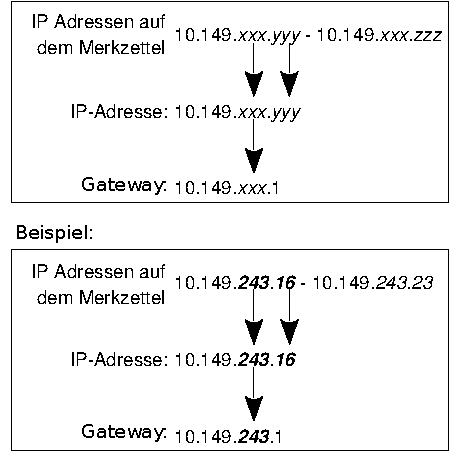
\includegraphics[width=\linewidth,keepaspectratio]{Bilder/IP_Gerneric}
		\end{minipage}
	\end{figure}

\newpage
\enlargethispage{20pt}


\begin{figure}[h]
	\raggedleft
	\vspace{-20pt}
	
\includegraphics[height=1cm,keepaspectratio]{Bilder/Windows_logo}
	\vspace{-30pt}
\end{figure}

\subsubsection*{Schritt für Schritt Anleitung Windows}

\paragraph*{Windows 10}
\begin{enumerate}
	\item Klicken Sie auf das Windowssymbol in der unteren linken Ecke und anschließend auf \emph{Einstellungen}
	\item Klicken Sie auf \textit{Netzwerk und Internet}. Scrollen Sie runter bis \textit{Netzwerk und Freigabecenter} und klicken auf diesen Punkt. Wählen Sie in der linken Spalte den Punkt \textit{Adaptereinstellungen ändern}. Sollten Sie diesen Punkt nicht finden können Sie auch in der Suchzeile rechts oben nach \glqq Adaptereinstellungen ändern\grqq suchen.
%	\begin{figure}[h!]
%	\centering
%		\begin{minipage}[c]{0.3\linewidth}
%			\centering
%			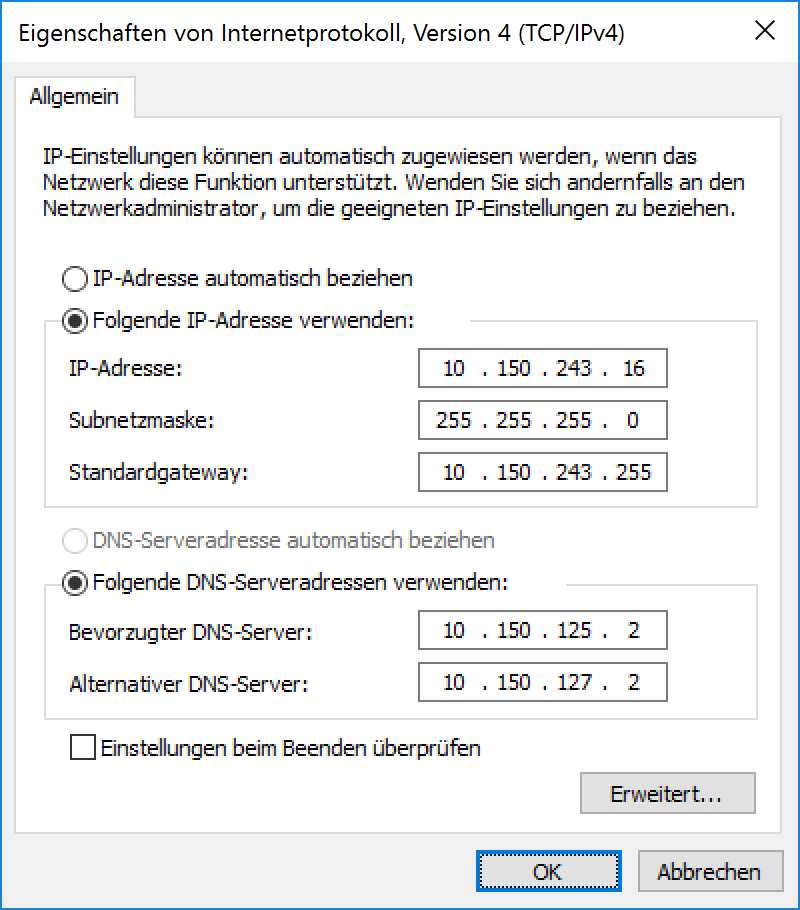
\includegraphics[width=0.9\linewidth,keepaspectratio]{Bilder/IP_Windows}
%			\caption{Beispielhafte Netzwerkeinstellungen unter Ubuntu Linux}
%			\vspace{-15pt}
%		\end{minipage}
%	\end{figure}

    \item Ihnen sollten nun mehrere Netzwerkverbindungen aufgelistet sein. Klicken Sie mit der \textbf{rechten} Maustaste auf \textit{Ethernet} und klicken Sie dann auf \textit{Eigenschaften}.
\end{enumerate}
$\rightarrow$ Weiter bei Punkt 5.


\begin{wrapfigure}[5]{R}{0.3\textwidth}
\centering
  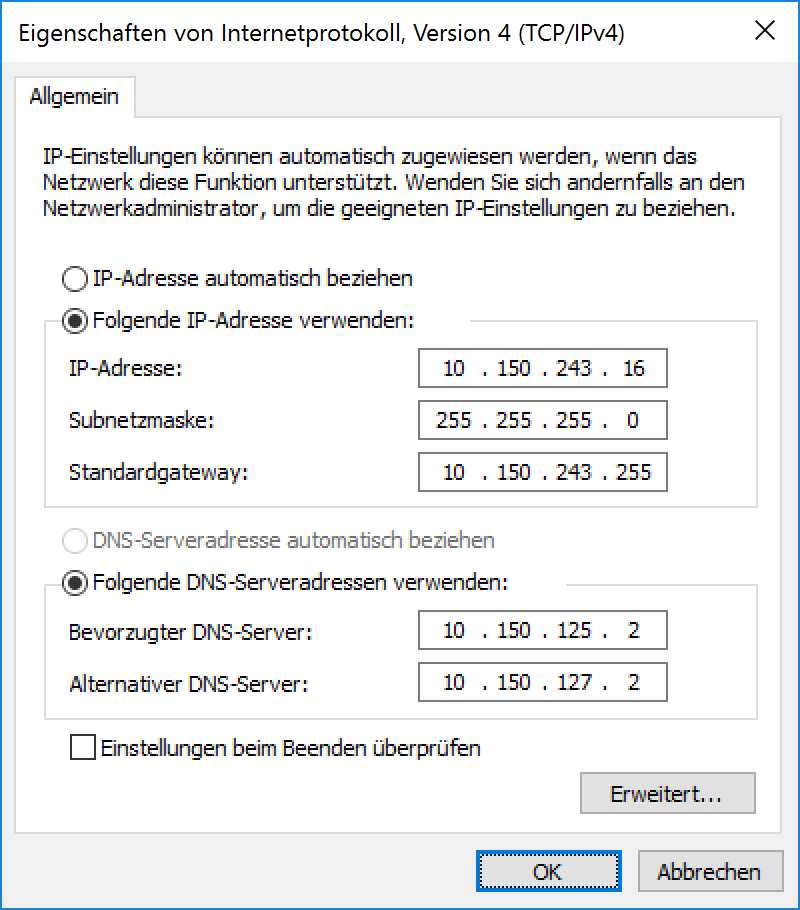
\includegraphics[width=0.3\textwidth]{Bilder/IP_Windows}
%  \caption{Bildunterschrift}
\end{wrapfigure}



\paragraph*{Windows 8}
\begin{enumerate}
	\item Öffnen Sie die Systemsteuerung, indem Sie die Windows-Taste drücken, \glqq Systemsteuerung\grqq  \ eingeben und ENTER drücken
	\item Wählen Sie unter Netzwerk und Internet den Punkt Netzwerkstatus und -aufgaben anzeigen.
    \item Nach Klick auf Netzwerkverbindungen verwalten wählen Sie im darauffolgenden Fenster durch einen Rechtsklick auf LAN-Verbindung deren Eigenschaften aus.
\end{enumerate}
$\rightarrow$ Weiter bei Punkt 5.



\paragraph*{Windows 8/10}
\begin{enumerate}
    \setcounter{enumi}{4}
    \item Markieren Sie den Eintrag \textit{Internetprotokoll Version 4 (TCP/IPv4)} (Windows Vista/7/8/10) bzw. Internetprotokoll  (TCP/IP) (Windows XP) und klicken Sie danach auf Eigenschaften.
    \item Jetzt geben Sie IP-Adresse, Subnetzmaske, Standardgateway und DNS Server ein. Die Adressen der DNS-Server lauten \textbf{10.150.127.2} und \textbf{10.150.125.2}, die Subnetzmaske \textbf{255.255.255.0}. Ihre jeweilige IP-Adresse steht auf einem Aufkleber auf Ihrer Anschlussbuchse bzw. auf dem Zettel, den Sie mit Ihrem Mietvertrag erhalten haben. Sollten Sie keinen Zettel mit Netzwerkdaten bekommen haben und der Aufkleber auf der Anschlussbuchse unlesbar sein, wenden Sie sich bitte an die Hausverwaltung oder besuchen Sie unsere Sprechstunde.
    \item Klicken Sie auf Erweitert und wählen im folgenden Dialog den Reiter DNS aus. Tragen Sie im Feld DNS-Suffix für diese Verbindung \textbf{stusta.mhn.de} ein.
    \item Bestätigen mit OK.
\end{enumerate}
$\rightarrow$ Weiter bei den Browsereinstellungen.



\pagebreak

\begin{figure}[t!]
	\raggedleft
	\vspace{-20pt}
	
\includegraphics[height=1cm,keepaspectratio]{Bilder/linux_logo_neu}
	\vspace{-30pt}
\end{figure}



\subsubsection*{Schritt für Schritt Anleitung Linux}

\begin{enumerate}
	\item Öffnen Sie die Netzwerkkonfiguration durch Klick auf \emph{System} $\rightarrow$ \emph{Einstellungen} $\rightarrow$ \emph{Netzwerkkonfiguration}.
	\item Markieren Sie nun im Reiter Kabelgebunden den entsprechenden Eintrag Ihrer Netzwerkkarte (im Normalfall \emph{eth0}) und klicken Sie auf den Button \emph{Bearbeiten}.
	\item Gehen Sie zum Reiter \emph{IPv4-Einstellungen} und setzen Sie Methode auf \emph{Manuell}.
	\item Unter \emph{Adressen} klicken Sie auf den Button \emph{Hinzufügen}.
	\begin{figure}[h!]
	\centering
		\begin{minipage}[c]{0.5\linewidth}
			\centering
			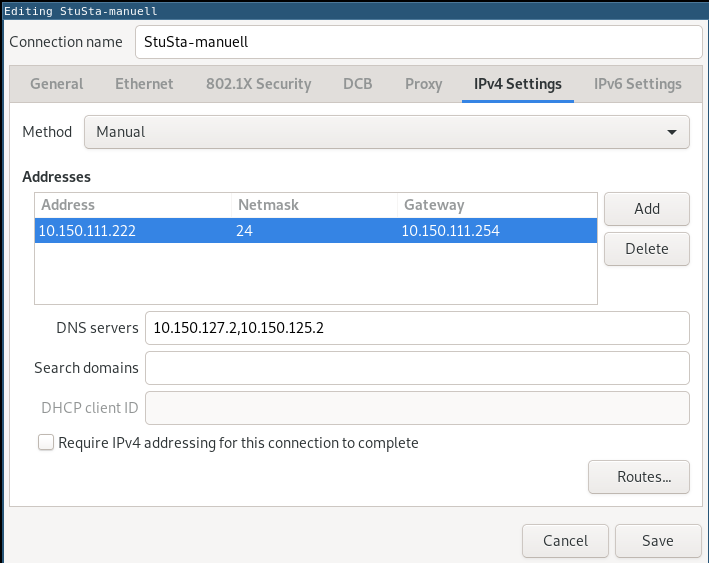
\includegraphics[width=0.9\linewidth,keepaspectratio]{Bilder/IP_Ubuntu_neu}
%			\caption{Beispielhafte Netzwerkeinstellungen unter Ubuntu Linux}
			\vspace{-15pt}
		\end{minipage}
	\end{figure}
	\item Jetzt geben Sie IP-Adresse, Subnetzmaske, Gateway, DNS und Suchdomäne ein. Die Adressen der DNS-Server lauten \textbf{10.150.127.2} und \textbf{10.150.125.2}, die Suchdomäne \textbf{stusta.mhn.de} und die Netzmaske \textbf{255.255.255.0}. Ihre jeweilige IP-Adresse steht auf einem Aufkleber auf Ihrer Anschlussbuchse bzw. auf dem Zettel, den Sie mit Ihrem Mietvertrag erhalten haben. Sollten Sie einen neuen Zettel benötigen, wenden Sie sich bitte an die Hausverwaltung oder besuchen Sie unsere Sprechstunde. Bestätigen Sie mit \emph{OK} und schließen Sie das Fenster für die Netzwerkeinstellungen.
\end{enumerate}

\paragraph*{Proxy global einstellen} ~\\
\\
Unter Linux haben Sie die Möglichkeit den Proxy global zu definieren, sodass dieser nicht extra für jedes Programm eingetragen werden muss.
\begin{enumerate}
	\item Öffnen Sie die Netzwerk-Proxy-Einstellungen durch Klick auf \emph{System} $\rightarrow$ \emph{Einstellungen} $\rightarrow$ \emph{Netzwerk-Proxy}.
	\item Hier markieren Sie ganz unten die Option \emph{Automatische Proxy-Konfiguration} und tragen bei URL für Auto-Konfiguration: \url{http://wpad.stusta.mhn.de/proxy.pac} ein. Schließen Sie das Fenster. 
\end{enumerate}



\newpage
\enlargethispage{20pt}



\begin{figure}[t!]
	\raggedleft
	\vspace{-20pt}
	
\includegraphics[height=1cm,keepaspectratio]{Bilder/apple_logo_neu}
	\vspace{-30pt}
\end{figure}
\subsubsection*{Schritt für Schritt Anleitung MacOS}
\begin{enumerate}
    \item Öffnen Sie die Netzwerkkonfiguration durch Klick auf \emph{Apfel} (oben links) und wählen dann \emph{Systemeinstellungen} $\rightarrow$ \emph{Netzwerk} aus.
    \item Markieren Sie nun das Netzwerkgerät \emph{Ethernet}.
    \item Setzen Sie das Feld \emph{IPv4 Konfigurieren} auf \emph{Manuell}.
    \item Jetzt geben Sie \textbf{IP-Adresse, Teilnetzmaske, Gateway, DNS-Server} und \textbf{Such-Domains} ein. Die Adressen der DNS-Server lauten \textbf{10.150.127.2} und \textbf{10.150.125.2}, die Such-Domains \textbf{stusta.mhn.de} und die Teilnetzmaske \textbf{255.255.255.0}. Ihre jeweilige IP-Adresse steht auf einem Aufkleber auf Ihrer Anschlussbuchse bzw. auf dem Internetkonfigurationsblatt, das Sie mit Ihrem Mietvertrag erhalten haben. Sollten Sie dieses Blatt nicht mehr finden, wenden Sie sich bitte an die Hausverwaltung oder besuchen Sie unsere Sprechstunde. Bestätigen Sie mit \emph{Anwenden}.
      \begin{figure}[h!]
      \centering
%      \vspace{-5pt}
        \begin{minipage}[c]{0.60\linewidth}
          \centering
          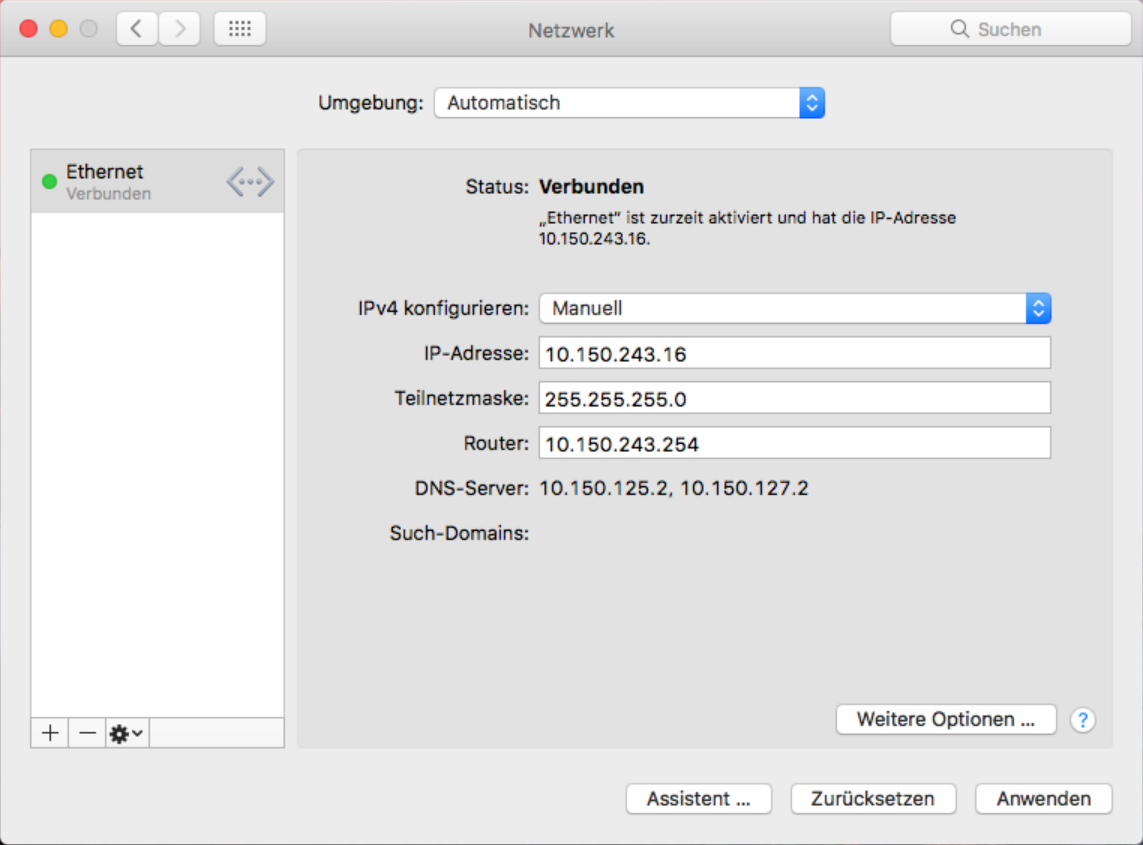
\includegraphics[width=0.9\linewidth,keepaspectratio]{Bilder/IP_MAC}
%          \caption{Beispielhafte Netzwerkeinstellungen unter Mac OS~X}
        \end{minipage}
      \vspace{-20pt}
      \end{figure}
\end{enumerate}
\vspace{-10pt}
\paragraph*{Proxy global einstellen}~\\
\\
Unter MacOS haben Sie die Möglichkeit den Proxy global zu definieren, sodass dieser nicht extra für jedes Programm eingetragen werden muss. Firefox benötigt allerdings trotzdem eine gesonderte Einstellungen (siehe Browsereinstellungen). %noch aktuelle info??

%\begin{wrapfigure}{r}{0.4\textwidth}
%  \vspace{-20pt}
%  \begin{center}
%    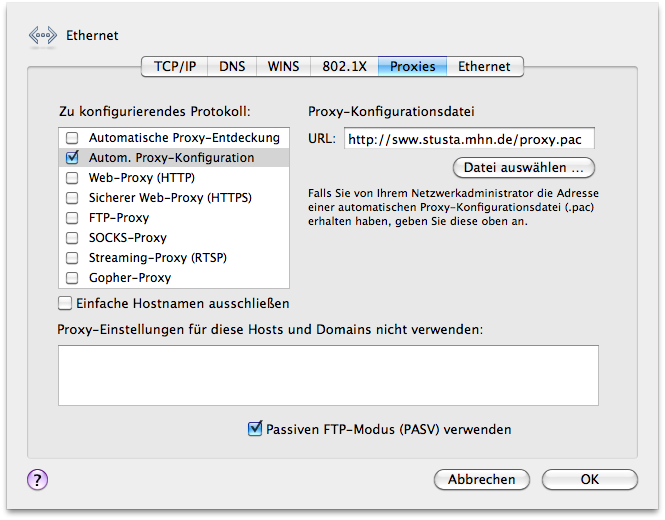
\includegraphics[width=0.48\textwidth,keepaspectratio]{Bilder/Proxy_MAC}
%  \end{center}
%  \vspace{-20pt}
%  \caption{Beispielhafte Proxyeinstellungen unter Mac OS~X}
%  \vspace{-10pt}
%\end{wrapfigure}
\begin{enumerate}%WTF 1. punkt???
    \item Öffnen Sie mit dem Button \emph{Weitere Optionen...} im voherigen Dialog die Detaileinstellungen und wechseln sie auf die Registerkarte \emph{Proxies}
    \item Setzen sie bei Zu konfigurierendes Protokoll vor Autom. Proxy-Konfiguration einen Hacken und tragen rechts bei URL \url{http://wpad.stusta.mhn.de/proxy.pac} ein. Schließen Sie die Detaileinstellungen mit OK und bestätigen Sie erneut mit Anwenden. Sie können die Netzwerkeinstellungen jetzt schließen.
\end{enumerate}
$\rightarrow$ Der Internetzugang ist jetzt fertig konfiguriert.

\newpage

\section*{Proxy-Konfiguration im Browser (nur Nicht-Mitglieder)}
\label{Proxy}

\begin{wrapfigure}{r}{0.5\textwidth}
	\vspace{-40pt}
	\begin{center}
		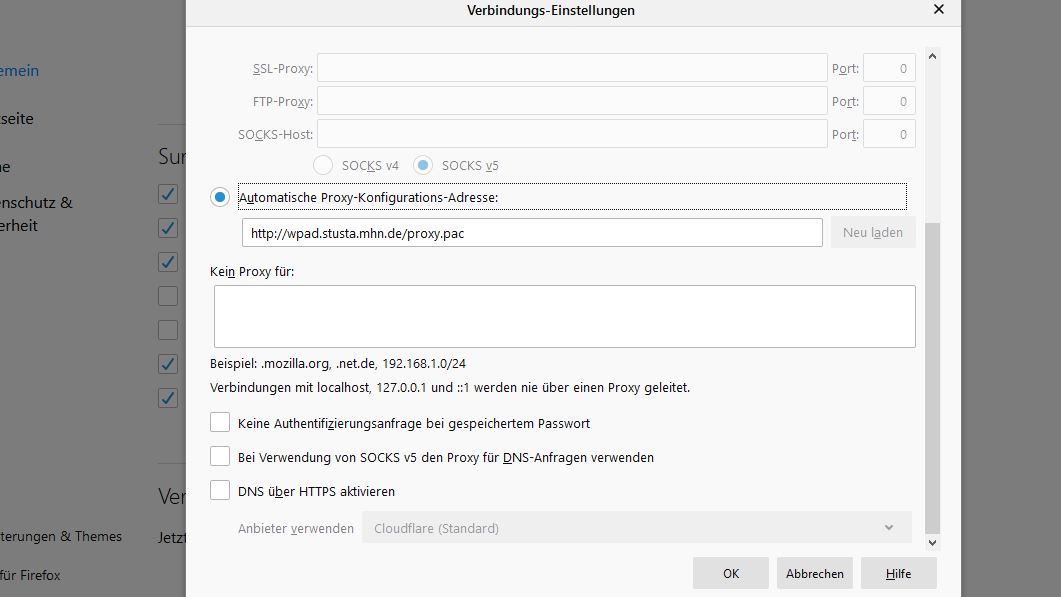
\includegraphics[width=0.5\textwidth,keepaspectratio]{Bilder/Firefox_neu_proxy}
	\end{center}
	%  \vspace{-20pt}
%	\caption{Eintragen des Proxyskripts in Mozilla Firefox}
	%  \vspace{-10pt}
\end{wrapfigure}

\subsection*{
\includegraphics[height=1.2cm,keepaspectratio]{Bilder/Firefox_35_logo} Mozilla Firefox}
\begin{enumerate}
	\item Klicken Sie auf die 3 übereinanderliegenden Striche in der rechten oberen Ecke, wählen Sie danach \emph{Einstellungen}
	\item Gehen Sie zum Punkt \emph{Verbindungs-Einstellungen} und wählen diesen aus.
	\item Markieren Sie den Punkt \emph{Automatische Proxy-Konfigurations-Adresse} und tragen Sie als Automatische Proxy-Konfigurations-URL: \\ \url{http://wpad.stusta.mhn.de/proxy.pac} ein.
	\item Bestätigen Sie mit OK .\\
	\\
	\\
\end{enumerate}





%\newpage
%\begin{wrapfigure}{r}{0.5\textwidth}
%	\vspace{-40pt}
%	\begin{center}
%		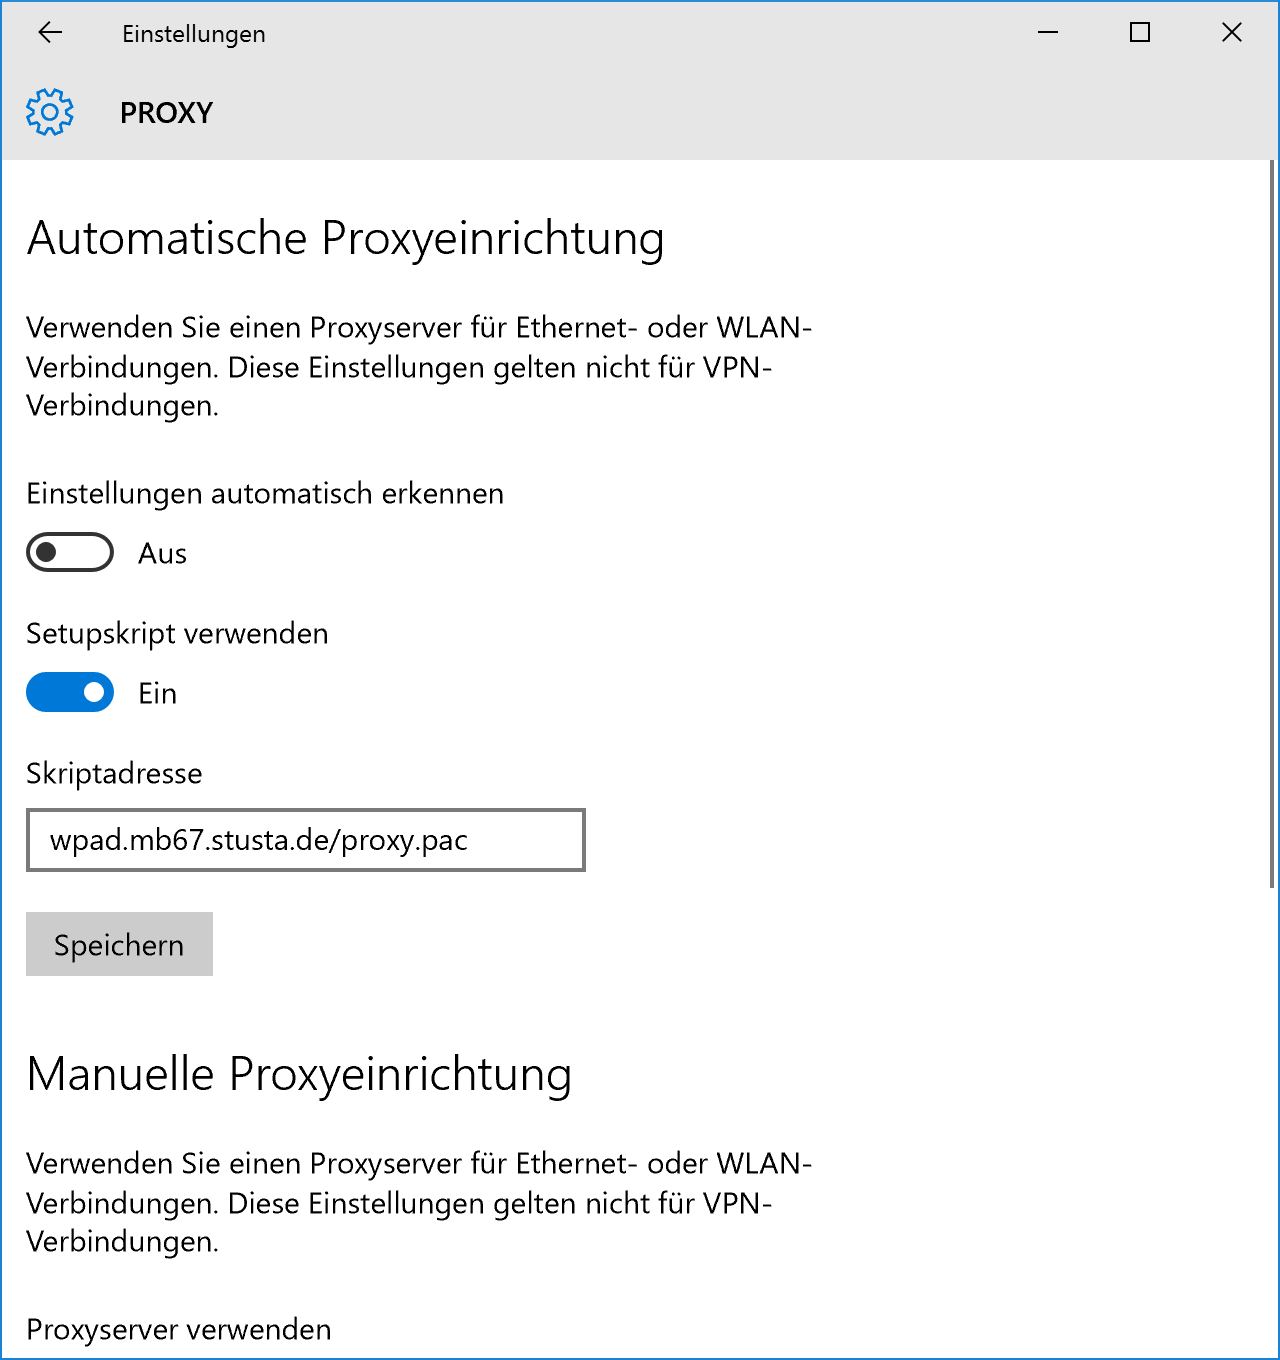
\includegraphics[width=0.5\textwidth,keepaspectratio]{Bilder/Proxy_Edge.png}
%	\end{center}
%	%  \vspace{-20pt}
%	\caption{Eintragen des Proxyskripts in Google Chrome}
%	%  \vspace{-10pt}
%\end{wrapfigure}
\subsection*{
\includegraphics[height=1.2cm,keepaspectratio]{Bilder/Chrome_2011_logo} Google Chrome}
\begin{enumerate}
	\item Chrome starten.
	\item Klicken Sie auf die 3 übereinanderliegenden Striche in der rechten oberen Ecke, wählen Sie danach \emph{Einstellungen}.
	\item Wählen Sie den Punkt \emph{Erweiterte Einstellungen anzeigen}.
	\item Klicken Sie auf \emph{Proxy-Einstellungen des Computers öffnen}.
	\\
	\\
\end{enumerate}
$\rightarrow$ Weiter bei Punkt 5 unter Microsoft Edge

\newpage
\begin{wrapfigure}{r}{0.5\textwidth}
	%  \vspace{-20pt}
	\begin{center}
		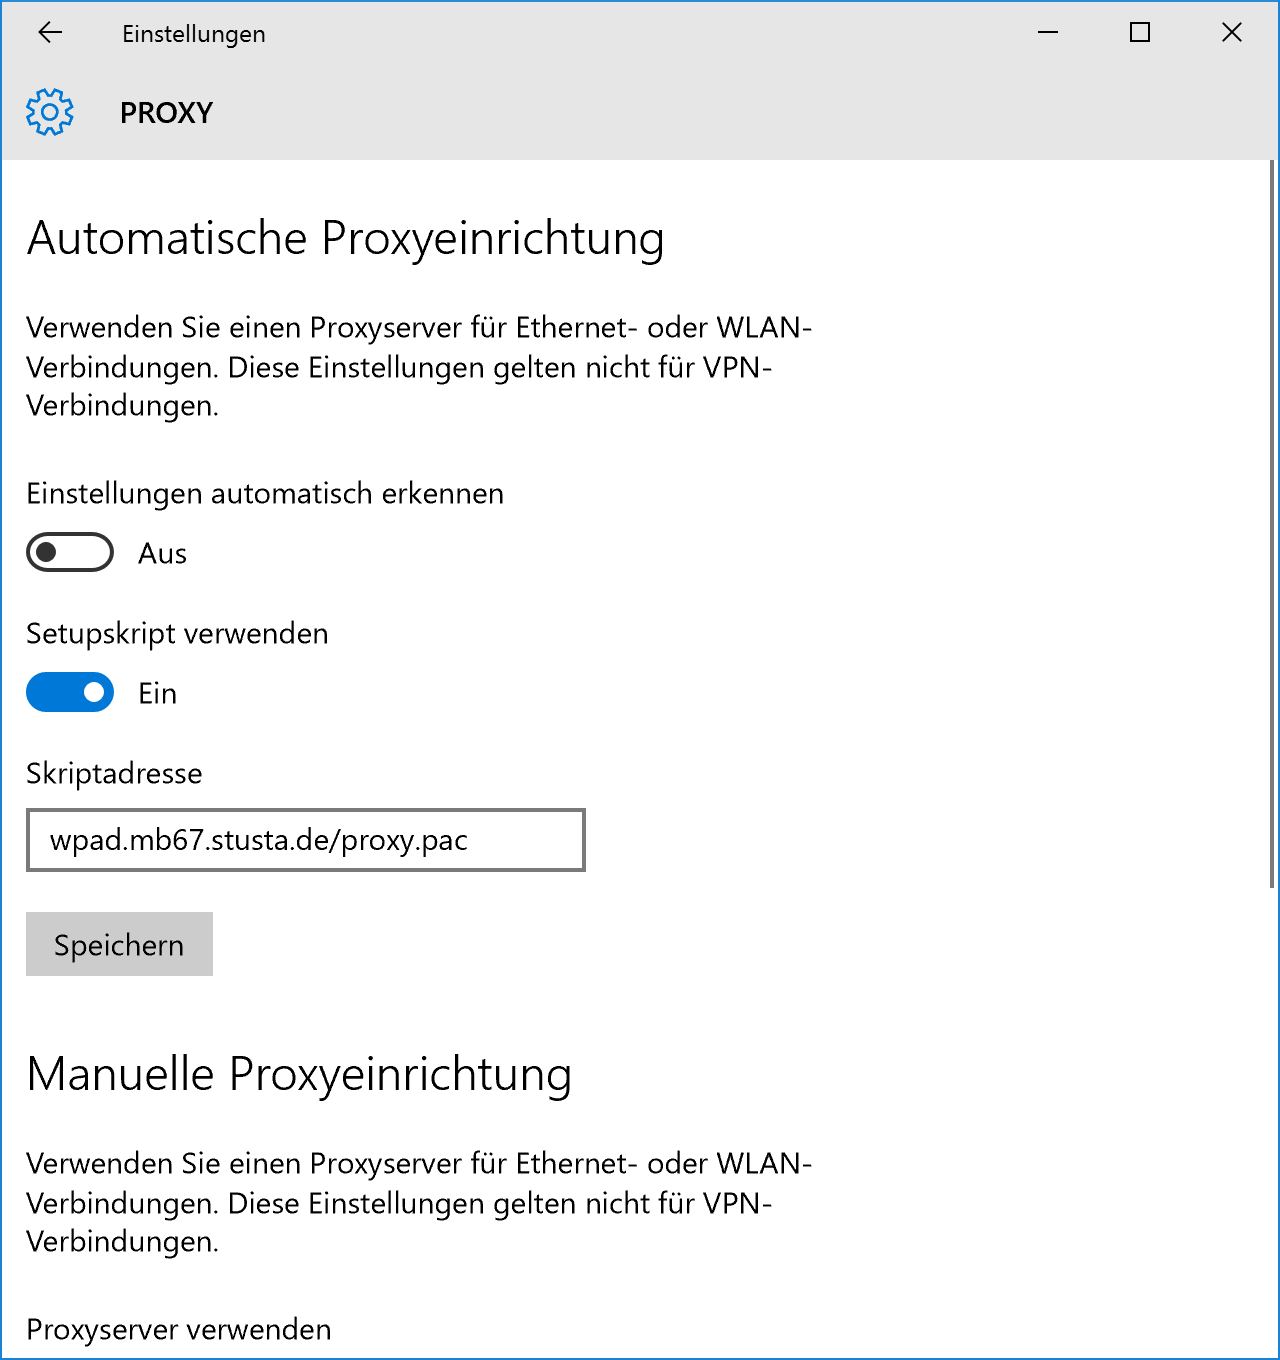
\includegraphics[width=0.5\textwidth,keepaspectratio]{Bilder/Proxy_Edge}
	\end{center}
	%  \vspace{-20pt}
%	\caption{Eintragen des Proxyskripts in Microsoft Edge}
	%  \vspace{-10pt}
\end{wrapfigure}

\subsection*{
\includegraphics[height=1.2cm,keepaspectratio]{Bilder/Mcrosoft_Edge_logo} Microsoft Edge}
\begin{enumerate}
	\item Microsoft Edge starten.
	\item Klicken Sie auf die 3 übereinanderliegenden Striche in der rechten oberen Ecke, wählen Sie danach \emph{Einstellungen}.
	\item Wählen Sie den Punkt \emph{Erweiterte Einstellungen anzeigen}.
	\item Klicken Sie auf \emph{Proxyeinstellungen öffnen}.
	\item Deaktivieren Sie die Option \emph{Einstellungen automatisch erkennen}.
	\item Wählen Sie \emph{Setupskript verwenden} und tragen Sie bei der Adresse \\ \url{http://wpad.stusta.mhn.de/proxy.pac} ein.
	\item Klicken Sie auf speichern und schließen Sie die geöffneten Fenster.
\end{enumerate}
$\rightarrow$ Der Internetzugang ist nun fertig konfiguriert.

%\newpage
%\begin{wrapfigure}{r}{0.5\textwidth}
%%  \vspace{-20pt}
%  \begin{center}
%    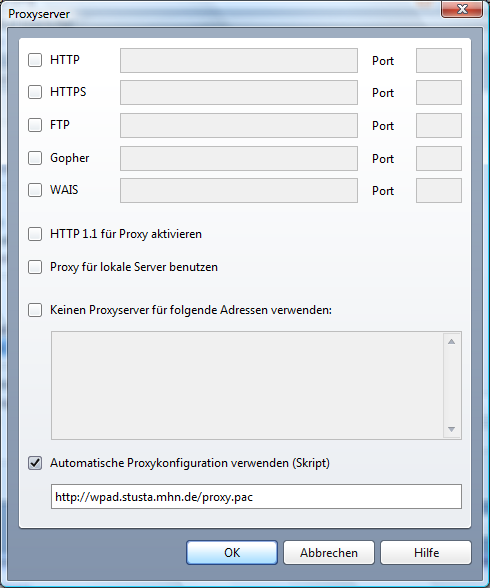
\includegraphics[width=0.5\textwidth,keepaspectratio]{Bilder/Proxy_Opera}
%  \end{center}
%%  \vspace{-20pt}
%  \caption{Eintragen des Proxyskripts im Opera}
%%  \vspace{-10pt}
%\end{wrapfigure}
%
%\subsection*{
\includegraphics[height=1.2cm,keepaspectratio]{Bilder/Opera_O} Opera}
%\begin{enumerate}
%    \item Opera starten.
%    \item Wählen Sie im Untermenü Extras den Punkt Einstellungen...
%    \item Wählen Sie im Reiter Erweitert auf der linken Seite die Kategorie Netzwerk und dann klicken Sie auf den Button Proxy.
%    \item Setzen Sie bei Automatische Proxykonfiguration verwenden (Skript) einen Haken und tragen Sie \\ \url{http://wpad.mb67.stusta.mhn.de/proxy.pac} ein.
%    \item Schließen Sie beide Fenster mit OK.
%\end{enumerate}
%$\rightarrow$ Der Internetzugang ist nun fertig konfiguriert.


\end{document}
